\documentclass[
	article,			
	12pt,				
	oneside,			
	a4paper,			
	english,			
	brazil,				
	sumario=tradicional
	]{abntex2}

\usepackage{lmodern}			
\usepackage[T1]{fontenc}		
\usepackage[utf8]{inputenc}		
\usepackage{indentfirst}		
\usepackage{nomencl} 			
\usepackage{color}				
\usepackage{graphicx}			
\usepackage{microtype}
\usepackage{lipsum}
\usepackage[brazilian,hyperpageref]{backref}
\usepackage[alf]{abntex2cite}
\usepackage{float}

\renewcommand{\backrefpagesname}{Citado na(s) página(s):~}

\renewcommand{\backref}{}

\renewcommand*{\backrefalt}[4]{
	\ifcase #1 %
		Nenhuma citação no texto.%
	\or
		Citado na página #2.%
	\else
		Citado #1 vezes nas páginas #2.%
	\fi}%

\titulo{Assalto de celulares por assaltantes disfarçados de entregadores de aplicativo na região do Grajaú - Zona Sul, São Paulo}
\tituloestrangeiro{}

\autor{
    \Large Centro Universitário Senac \\
    Bacharelado em Ciência da Computação 
\\[0.75cm]
\normalsize João Watson, Lucas Henrique, Murilo Cantante \\
\normalsize Priscila Wolff, Ricardo Hemmel, Thiago Pereira
}

\local{São Paulo}
\data{São Paulo, 30 de Maio 2022}

\definecolor{blue}{RGB}{41,5,195}

\makeatletter
\hypersetup{
        %pagebackref=true,
		pdftitle={\@title}, 
		pdfauthor={\@author},
        pdfsubject={Roubo de celulares no centro da cidade de São Paulo},
        pdfcreator={LaTeX with abnTeX2},
		pdfkeywords={roubo de celulares}{drogas}{operação civil}, 
		colorlinks=true,       		% false: boxed links; true: colored links
        linkcolor=blue,          	% color of internal links
        citecolor=blue,        		% color of links to bibliography
        filecolor=magenta,      	% color of file links
		urlcolor=blue,
		bookmarksdepth=4
}
\makeatother

\makeindex

\setlrmarginsandblock{3cm}{3cm}{*}
\setulmarginsandblock{3cm}{3cm}{*}
\checkandfixthelayout

% O tamanho do parágrafo é dado por:
\setlength{\parindent}{1.3cm}

\setlength{\parskip}{0.2cm}

\SingleSpacing

\begin{document}

\selectlanguage{brazil}
\frenchspacing 
\maketitle

\begin{resumoumacoluna}
    
    Trata-se de um artigo com base no pensamento computacional, no qual possui o objetivo de 
    informar sobre como ocorre o roubo de celulares no centro da cidade de São Paulo e como
    eles contribuem para o mercado ilegal, além de causar uma alta insegurança e um alto prejuízo ao
    cidadão brasileiro. Alguns casos ocorrem devido ao vício em drogas, fazendo com que o
    infrator roube celulares para comprar mais drogas. A solução encontrada para auxiliar na
    amenização desses casos é executar uma operação civil na região.
    
    \vspace{\onelineskip}
    
    \noindent
    \textbf{Palavras-chave}: roubo de celulares. drogas. operação civil.
\end{resumoumacoluna}

\textual

\newpage
% Priscila Wolff
\section{Introdução}

Apesar de ser um delito bastante conhecido, o roubo de celulares possui em sua 
essência algumas características relevantes que merecem atenção, e neste artigo,
iremos abordar os pontos na região do Grajaú na cidade de São Paulo, analisando
assaltos no qual o infrator disfarça-se de entregador de aplicativo em específico.

Previsto no Título II, dos crimes contra o patrimônio, do Código Penal Brasileiro,
o crime de roubo possui as mesmas características do crime de furto, porém, quando 
há o emprego de grave ameaça, de violência ou outro meio que impossibilite a 
resistência da vítima, fatores estes, empregados pelo agente para que a vítima 
entregue o bem, está configurado o presente crime.


\newpage
% Ricardo Hemmel
\section{Objetivo}

    \subsection{Objetivos Gerais}

        Este artigo visa estabelecer uma clara relação entre o roubo de aparelhos 
        celular e os serviços de delivery, e como isso interfere na segurança pública
        tendo como referência a região do Grajaú. Essa pesquisa se desenvolve analisando
        esses casos e formas de contornar  essa situação no intuito de melhorar a 
        situação dos moradores da região  escolhida. Dessa modo, informar o leitor 
        sobre o problema social da região do Grajaú  

    \subsection{Objetivos Específicos}


\newpage
% Murilo Cantante
\section{Metodologia}

    Através do pensamento computacional, foi possível concluir que \ldots


\newpage
% Thiago Pereira
% Lucas Henrique
\section{Discussão}

    % Aqui deve ser discutido o problema tratado pelo trabalho, de modo fundamentado,
    % com citações diretas e indiretas. Essa discussão deve ser feita de modo que
    % contenha informações suficientes para o desenvolvimento do objetivo de trabalho.
    Abaixo será discutido e analisado o que pode ser feito para diminuir a alta taxa de
    roubos no Grajaú, baseando-se em estatísticas e notícias deste e de outros bairros em 
    situações semelhantes da cidade de São Paulo.

    Esta seção foi separada em três tópicos: Origem, Dados e estatísticas e Sugestões de melhora.

    \subsection{Origem}

        Com a flexibilização da quarentena devido ao Covid-19 e a popularização de aplicativos
        e serviços de entrega de alimentos, os casos de assaltos envolvendo assaltantes 
        disfarçando-se de entregadores de aplicativos começaram a aumentar 
        
        Devido à sua valorização, uma das coisas que os assaltantes mais procuram roubar é o
        celular, pois além de seu preço, é fácil de ser transportado e quando a vítima está
        distraída com ele, torna-se ainda mais fácil de realizar o assalto.
        
        Outro fator que faz o celular ser prioridade aos assaltantes é a quantidade de informações
        que podem ter dentro dele, como dados bancários, senhas e contas, podendo ter muito mais
        lucro ao roubar a vítima.

        Além da facilidade de ser transportado e de ser um produto muito valorizado, há também a
        baixa penalidade para quem rouba, para furtos a penalidade é de 1 a 4 anos de reclusão e 
        multa, e para assaltos é de 4 a 10 anos além da multa.

    \subsection{Dados e estatísticas}

        \subsubsection{Com que frequência ocorrem os roubos}
        Segundo a notícia feita pelo programa jornalístico SP1 e publicada no site G1 - Globo,
        no dia 19 de Maio de 2022, foram em todo o estado 26.484 furtos nos dois primeiros 
        meses do ano e 34.338 roubos no mesmo período, de acordo com dados dos boletins de 
        ocorrência. Este levantamento foi feito pela GloboNews. A notícia também apresenta que
        a cada hora 42 celulares são furtados ou roubados no estado de São Paulo. Grande parte
        das vítimas deste tipo de crime são pedestres no período da noite na cidade de São Paulo.
        Na capital, encontra-se o Grajaú como um dos bairros que possui os maiores números de ocorrências.

        O programa jornalístico também informa sobre um pacote de medidas preventivas
        do governo do estado de São Paulo, com o intuito de inibir a onda de ocorrências
        envolvendo assaltantes disfarçados de entregadores de aplicativos, realizando mais
        abordagens aos motociclistas e parcerias às empresas dos respectivos aplicativos para
        uma fiscalização mais efetiva.
        % https://g1.globo.com/sp/sao-paulo/noticia/2022/05/19/42-celulares-sao-roubados-ou-furtados-por-hora-no-estado-de-sp-em-janeiro-e-fevereiro.ghtml
        % Data 19 de Maio, 2022
        % Título: 42 Celulares são roubados ou furtados por hora no estado de São Paulo em Janeiro e Fevereiro
        % Autor: G1 - Globo, SP1 (Eu acho)

        \subsubsection{Onde se concentram os roubos}
        Há dados sobre onde mais se concentram os roubos de celulares no estado de São 
        Paulo no jornal Folha de São Paulo. Segundo os escritores Alfredo Henrique e William
        Cardoso, a volta do trabalho no início da noite é o horário no qual se corre o maior
        risco de ter o celular roubado na capital paulista, o perigo é maior para os moradores
        das periferias, onde estão os bairros que lideram nesse tipos de crime.

        Um levantamento feito pela reportagem analisou que foram registrados mais de 89.000
        boletins de ocorrência em 2021, constatando que no período entre 19h e 21h59 concentra
        1 em cada 4 roubos de celular (26,5\% das ocorrências).
        
        Na zona sul de São Paulo, bairros como Capão Redondo, Campo Limpo, Jardim Ângela,
        Jardim São Luís, e inclusive o Grajaú, onde ficam 6 dos 10 distritos policiais com
        mais assaltos em que celulares foram roubados, são as regiões com maior incidência
        do crime.

        \begin{figure}[H]
            \centering
            \textbf{Mapa dos Roubos de Celular em São Paulo}
            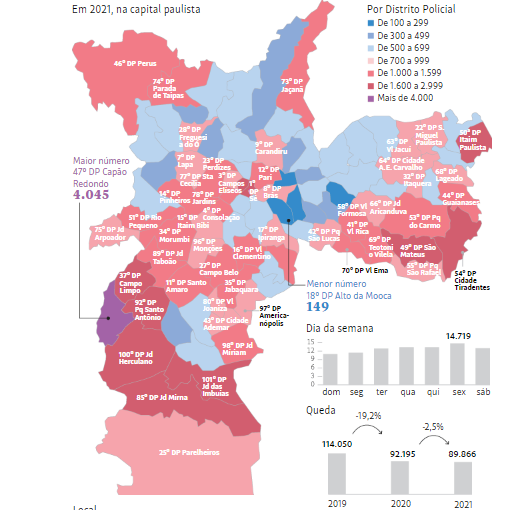
\includegraphics[scale=0.7]{img/mapa_dos_roubos_de_celular_em_sp.png}
            \caption{Fonte: Gráfico feito pela Folha S. Paulo, com dados da Secretaria da Segurança Pública do Estado de São Paulo}
        \end{figure}

        Observando os dados gerais, os casos de roubos de celular na capital paulista caíram
        de 114.050 para 92.195, entre 2019 e 2020, e para 89.866 em 2021. É possível observar
        também que grande parte dos roubos ocorrem na zona sul de São Paulo em relação às
        outras regiões da capital.
        % https://www1.folha.uol.com.br/cotidiano/2022/02/roubo-de-celular-se-concentra-na-volta-para-casa-e-na-periferia-de-sp.shtml
        % Data: 25 fev. 2022
        % Autores: Alfredo Henrique, William Cardoso
        % Título: Roubo de celular se concentra na volta para casa e na periferia de SP

    \subsection{Sugestões de melhora}

        De acordo com um especialista em segurança citado pelo programa jornalístico SP1, no dia 
        19 de Maio de 2022, há diversas coisas que podemos fazer para se proteger em caso de
        roubo de celular. "A primeira e mais simples é a senha. Não podem ser fáceis, dedutíveis
        ou estarem anotadas no celular. O que tem acontecido é roubo de celular quando ele está
        desbloqueado, seja por motoristas presos no celular ou pedestres utilizando-o na mão. O
        telefone na mão já é a primeira barreira derrubada, permitindo que os bandidos acessem
        nossos dados e até contas bancárias. Também todos nós devemos estar preparados para este 
        acidente. Quais são os telefones dos bancos que você tem de ligar? No momento de nervosismo,
        é importante ter esse roteiro na bolsa, no porta-luvas do carro, em casa, para você chegar
        e poder avisar que foi roubado.", o especialista afirma.
        % https://g1.globo.com/sp/sao-paulo/noticia/2022/05/19/42-celulares-sao-roubados-ou-furtados-por-hora-no-estado-de-sp-em-janeiro-e-fevereiro.ghtml

        Como sugestão de melhora, é possível realizar uma regularização para entregadores de
        aplicativo e aumentar as patrulhas policiais, evitando a possibilidade de assaltantes 
        se disfarçarem e facilitando a fiscalização para as autoridades. Alguns exemplos de 
        fiscalização que podem ser feitas são nos registros dos entregadores nos aplicativos, 
        dando mais recursos para poder distinguir entre quem está trabalhando e quem está se 
        disfarçando para diminuir suspeitas. Outra coisa que pode ser feita também é dar uma 
        formalização ao trabalho de entregador de aplicativo, possibilitando até mesmo a 
        utilização da placa para serviços e aluguéis ao invés da placa para veículos particulares.



\newpage
% João Watson
\section{Considerações finais}

    Ao decorrer desta pesquisa e considerando todos os pontos estudados e analisados,
    foi possível estabelecer uma relação entre o roubo de aparelhos celular e a
    crescente demanda de serviços de delivery. 

    Com o inicio pandemia e a crescente demanda de serviços de delivery, 
    fez com que a classe dos entregadores  crescesse como nunca antes visto, 
    esse fenômeno se deu pelo grande desemprego gerado pela Covid e a má 
    administração do governo vigente, juntamente com a facilidade de acesso aos 
    aparelhos celulares e internet domestica as pessoas passaram a pedir comida 
    e outros produtos com muito mais frequência, desde alimentos prontos, fast 
    food, mercado e até mesmo produtos farmacêuticos.

    Porem essa tendencia não diminuiu mesmo com o flexibilização da circulação 
    e a diminuição dos casos pois a população se acostumou com as facilidades 
    que esse tipo de serviço prove. Com as pessoas voltando as ruas,
    a grande quantidade de motoboys e a sucateamento da segurança publica, criou-se um cenário onde
    assaltantes disfarçados de entregadores cometem crimes contra o cidadão focando principalmente em 
    celulares sendo esse o item mais visado e rentável.

    Mostramos como fica cada vez mais vital a necessidade de regularização
    da profissão dos entregadores de aplicativo, para que, tanto o cidadão
    quanto os prestadores de serviço tenham mais segurança em seu dia a dia.

\postextual

\newpage

\bibliography{../referencias}
\noindent
HENRIQUE, Alfredo e CARDOSO, William. Roubo de celular se concentra na volta para casa e na periferia de SP, 25 de Fevereiro de 2022. 
Disponível em: <https://www1.folha.uol.com.br/cotidiano/2022/02/roubo-de-celular-se-concentra-na-volta-para-casa-e-na-periferia-de-sp.shtml> 
\\ \\
42 Celulares são roubados ou furtados por hora no estado de São Paulo em Janeiro e Fevereiro. G1 - Globo, 19 de Maio de 2022.
Disponível em: <https://g1.globo.com/sp/sao-paulo/noticia/2022/05/19/42-celulares-sao-roubados-ou-furtados-por-hora-no-estado-de-sp-em-janeiro-e-fevereiro.ghtml>


\end{document}
